\documentclass[11pt, oneside]{article}   	% use "amsart" instead of "article" for AMSLaTeX format
\usepackage{fullpage}
\usepackage{graphicx}
\usepackage{amssymb}

\title{Brief Article}
\author{The Author}
%\date{}							% Activate to display a given date or no date

\begin{document}
%\maketitle

\section{Mapping cylinder to 4 sides of cube}   

\begin{center}
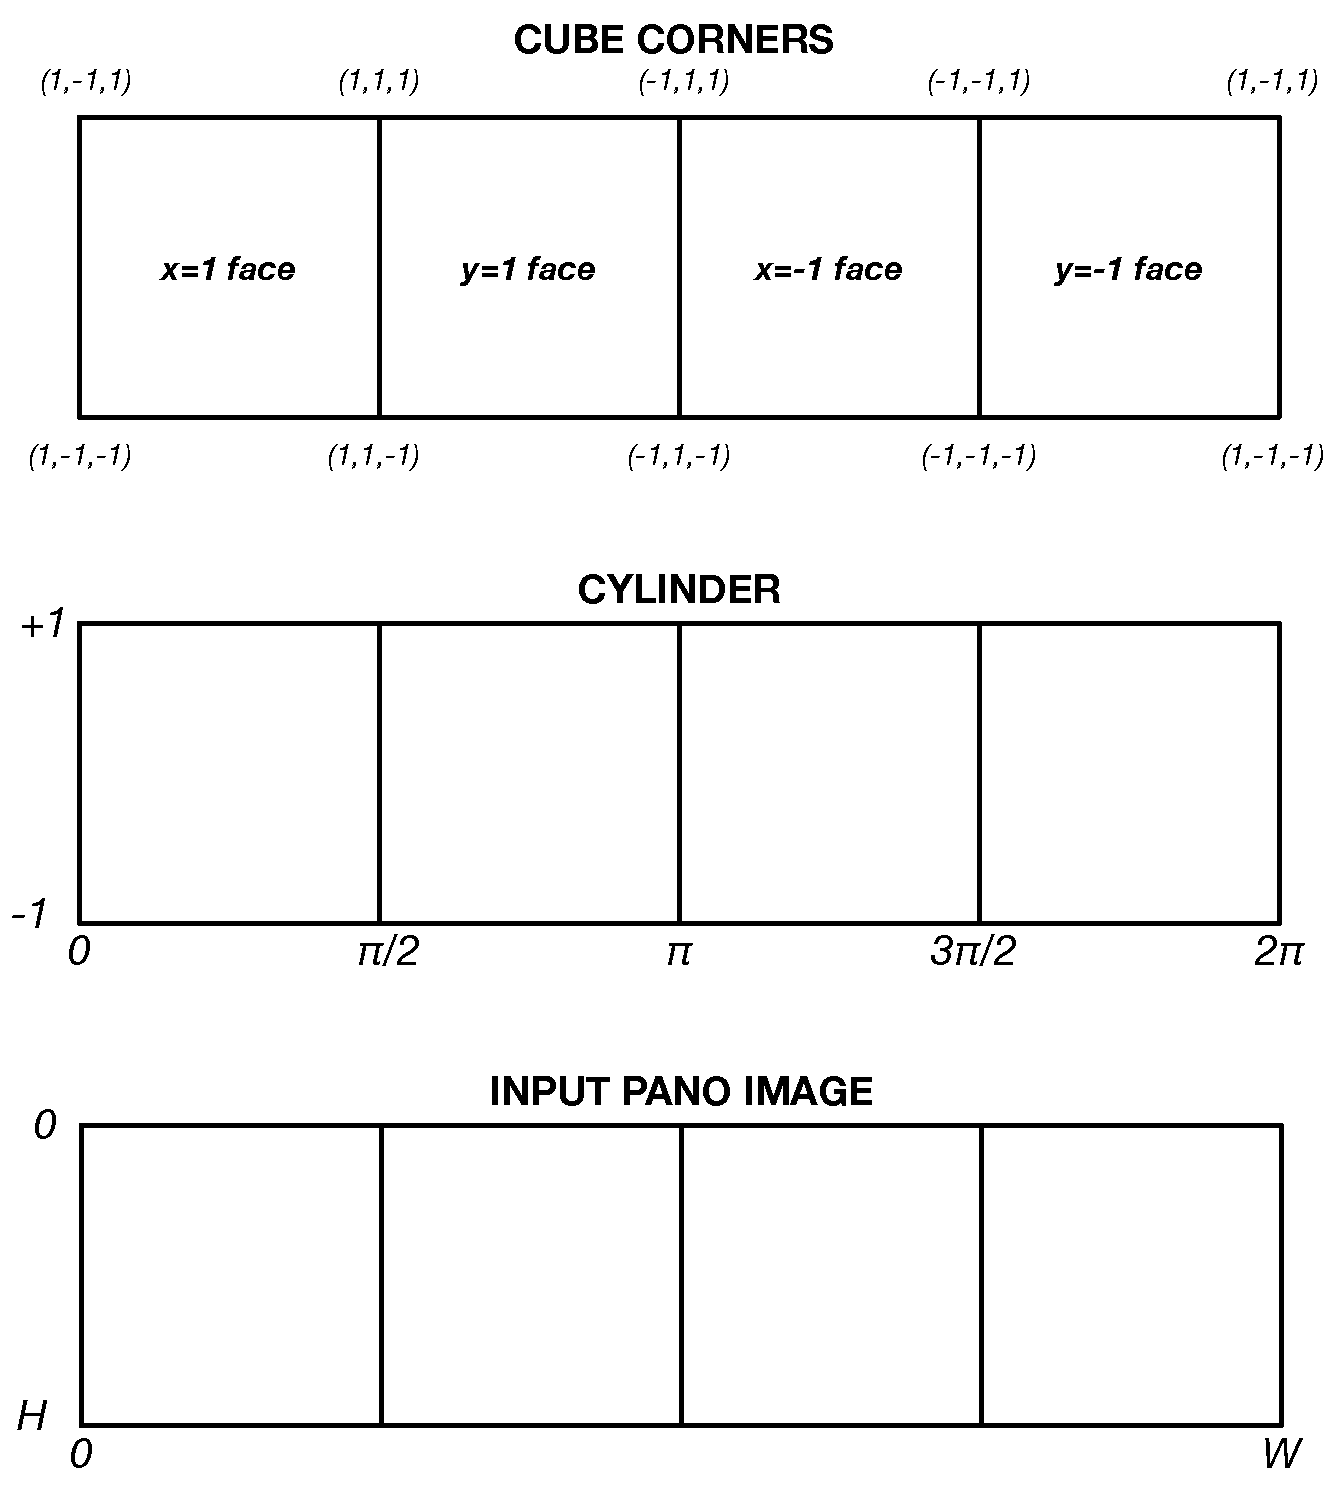
\includegraphics[width=0.6\textwidth]{cube_cylinder} 
\end{center}      
   
Given the cylinder $x^2 + y^2 = 1$ inscribed inside a $2 \times 2 \times 2$ cube
centered at the origin, we can project the cylindrical panorama onto the corresponding
four faces of the cube as follows.
For every pixel in the output image we cast a ray from the cube's center at $(0,0,0)$
through the corresponding point on one of the cube's faces and determine where that
ray intersects the cylinder. We then map this point on the cylinder to the corresponding
point in the input image and (bilinearly) sample the input image at the point. 
The resulting pixel color is assigned to the current output pixel.

We parameterize the ray emanating from 
the cube's center $(0,0,0)$ through a point $(u,v,w)$ on a face of the cube as
\begin{equation}
  \mathbf{r}(t) = (0,0,0) + t\cdot(u,v,w). \label{eq:r}
\end{equation}
This ray intersects the cylinder where
\begin{equation}
  (ut)^2 + (vt)^2 = 1.
\end{equation}
Solving we get $t = 1/\sqrt{u^2 + v^2},$ which we plug back into Equation~\ref{eq:r} and
get the cylindrical point
\begin{equation}
  \mathbf{p} = (x,y,z) = \frac{(u,v,w)}{\sqrt{u^2 + v^2}}. \label{eq:p-cyl}
\end{equation}
In cylindrical coordinates we have
\begin{eqnarray}
\mathbf{p} = \left(\theta, z\right), \ \ \ 
  \theta = \mbox{atan2}\left(y,x\right) + \pi/4. \label{eq:theta}
\end{eqnarray}
We added $\pi/4$ to $\theta$ so that the left edge of the image corresponds to
the left edge of the cube's $x = 1$ face (instead of the middle of the face);
Then we adjust for the appropriate image ``wrap-around:''
\begin{equation}
\theta' = \left\{\begin{array}{ll}
  \theta        & \theta \geq 0 \\
  \theta + 2\pi & \theta < 0
  \end{array}\right.
\end{equation}
Now the left edge of the input image corresponds to the left edge of the output image.
The resulting pixel coordinate in the input image is
\begin{equation}
(r,c) = \left(\frac{H}{2}\left(z + 1\right),\ \frac{W}{2\pi}\cdot \theta'\right).
\end{equation}




\begin{verbatim}
for row = 0 .. outImage.H-1 {
    for col = 0 .. outImage.W-1 {
       s = 4.0*col/outImage.W
       face = floor(s)  // face = 0,1,2,3
       f = s - face     // f = frac(s)
       if face == 0 {   // (u,v,w) = point on cube
           u = 1
           v = 2*f - 1
       } else if face == 1 {
           u = 1 - 2*f
           v = 1
       } else if face == 2 {
           u = -1
           v = 1 - 2*f
       } else {
           u = 2*f - 1
           v = -1
       }
       w = 2.0*row/outImage.H - 1
       (x,y,z) = (u,v,w)/sqrt(u*u + v*v) // project onto cylinder
       theta = atan2(y,x) + pi/4;        // cyl. coords, -3pi/4 <= theta <= 5pi/4
       if theta < 0                      // map to [0,2*pi)
           theta += 2*pi
       r = inImage.H*(z + 1)/2.0         // map to input pixel
       c = imImage.W*theta/(2*pi)
       outImage(row,col) = inImage.sample(r,c)
     }
}
\end{verbatim}

\section{Mapping sphere to 6 sides of cube}  

\begin{center}
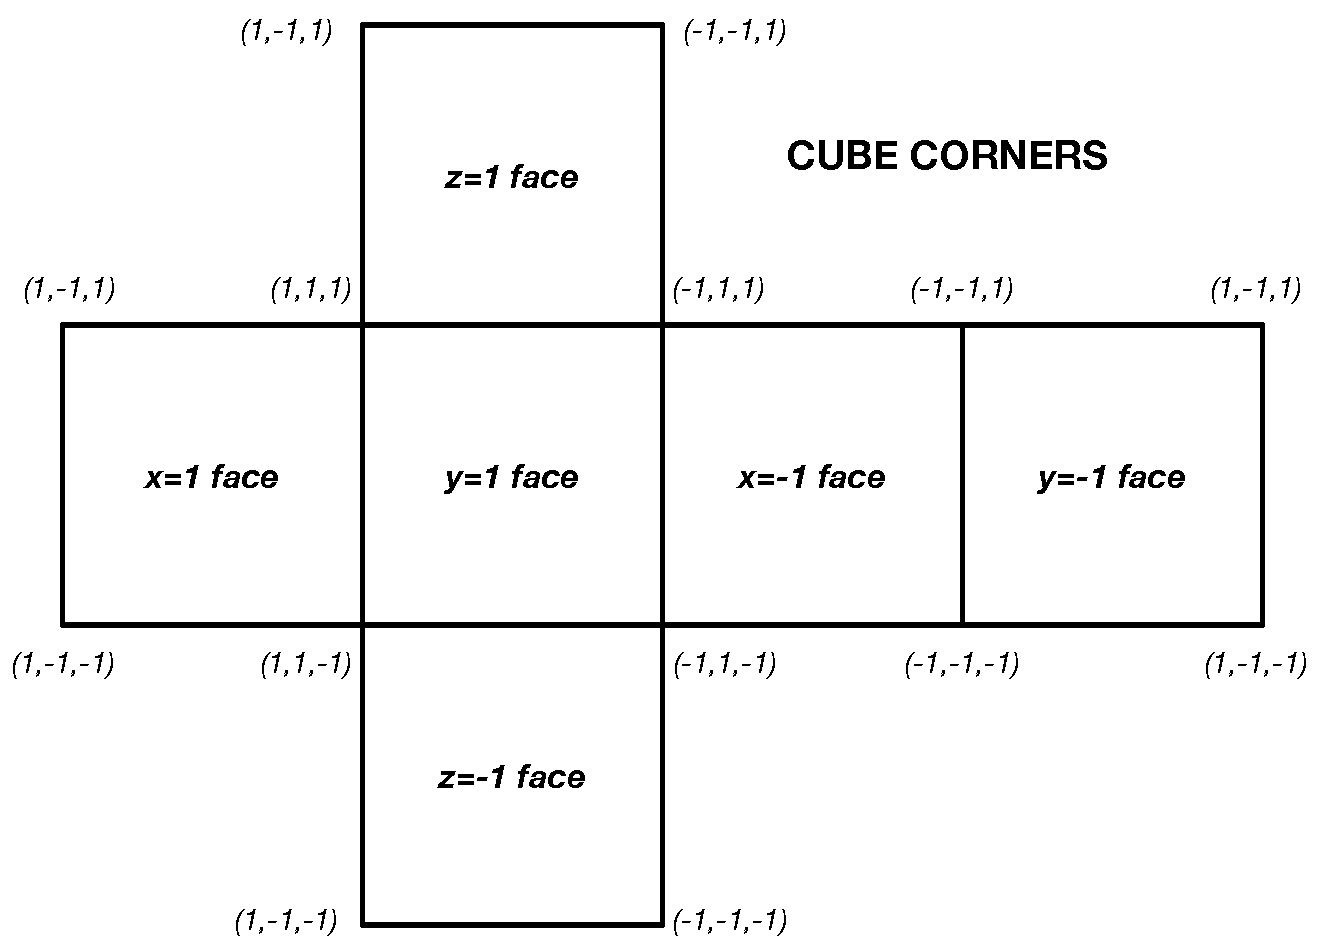
\includegraphics[width=0.6\textwidth]{cube_sphere} 
\end{center}      

Given the sphere $x^2 + y^2 + z^2= 1$ inscribed inside a $2 \times 2 \times 2$ cube
centered at the origin, we can project the spherical panorama onto the corresponding
four faces of the cube as follows.
For every pixel in the output image we cast a ray from the cube's center at $(0,0,0)$
through the corresponding point on one of the cube's faces and determine where that
ray intersects the sphere. We then map this point on the sphere to the corresponding
point in the input image and (bilinearly) sample the input image at the point. 
The resulting pixel color is assigned to the current output pixel.

We parameterize the ray emanating from 
the cube's center $(0,0,0)$ through a point $(u,v,w)$ on a face of the cube 
and find where it intersects the unit sphere. We use the mapping defined at
\begin{verbatim}
http://mathproofs.blogspot.com/2005/07/mapping-cube-to-sphere.html
\end{verbatim}
yielding
\begin{eqnarray}
x &=& u\sqrt{1 - \frac{v^2}{2} - \frac{w^2}{2} + \frac{v^2 w^2}{3}}, \\
y &=& v\sqrt{1 - \frac{w^2}{2} - \frac{u^2}{2} + \frac{w^2 u^2}{3}}, \\
z &=& w\sqrt{1 - \frac{u^2}{2} - \frac{v^2}{2} + \frac{u^2 v^2}{3}}.
\end{eqnarray}
We convert $(x,y,z)$ to the spherical coordinate $(\theta, \phi)$ where
the azimuthal angle is
\begin{equation}
\theta = \mbox{atan2}\left(y,x\right)
\end{equation}
and the elevation angle is
\begin{equation}
\phi = \mbox{atan2}\left(\sqrt{x^2+y^2},\ z\right).
\end{equation}

\pagebreak

We divvy up the output image into $3 \times 4 = 12$ squares where only 6 of the
squares actually map to the actual faces of the cube:
\begin{center}
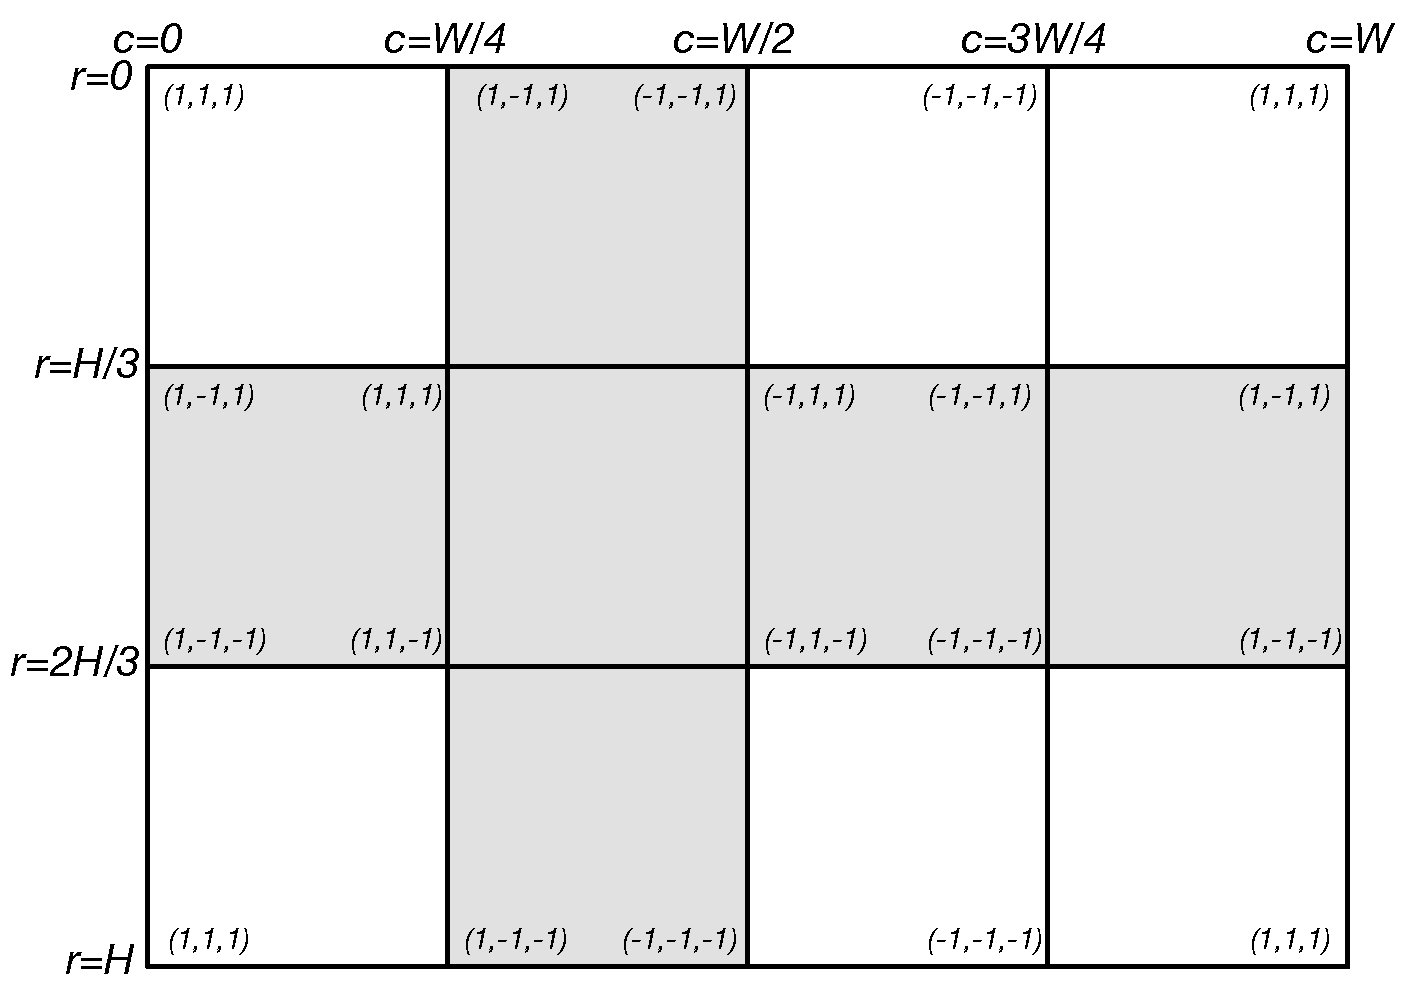
\includegraphics[width=0.6\textwidth]{cube-coords} 
\end{center}      
We pick $(u,v,w)$ coordinates for the unused corners so that the image has a toroidal topology.

\begin{verbatim}
for row = 0 .. outImage.H-1 {
    for col = 0 .. outImage.W-1 {
       a = 4.0*col/outImage.W
       b = 3.0*row/outImage.H
       (i,j) = (floor(a),floor(b))            // map to one of 12 squares
       (s,t) = (a - i, b - j)                 // uvw interpolation values
       (u,v,w) = bilerp(corners[j][i]), s,t)  // get cube coords w/in square
       (x,y,z) = cubeToSphereCoords(u,v,w)   
       (theta,phi) = cartesianToSpherical(x,y,z)
       r = theta*inImage.W/(2*pi)
       c = (phi + pi/2)*inImage.H/pi
       outImage(row,col) = inImage.sample(r,c)
     }
}
\end{verbatim}


\end{document}  